\documentclass[12pt]{article}

\title{Informe Tarea 2}

\author {Ronald Cardona
\and Anderson Grajales
\and Sebastian Valencia
\and Julian Sanchez}
\usepackage{graphicx}
\begin{document}
    
    \maketitle

    
    
    \section{Series de Taylor para aproximar funciones}
    Una técnica de aproximación es de poco valor sin alguna idea de su precisión.
    Para medir la precisión de una aproximación al valor de una función $f(x)$ mediante 
    un polinomio de Taylor $P_{n}(x)$, puede estar el concepto de residuo, que se define así:

    \begin{center}
        \begin{math}
            f(x) = P_{n} + R_{n}(x)
        \end{math}
    \end{center}

    Siendo $f(x)$ el valor exacto, $P_{n}(x)$ el valor aproximado y $R_{n}(x)$ el resto. El teorema
    de Taylor es un procedimiento general para estimar el residuo de un polinomio de Taylor. El residuo
    dado en el teorema se llama fórmula del residuo de Lagrange.
    Los polinomios de Taylor y de Maclaurin pueden usarse para aproximar el valor de una función en un
    punto específico. Al aplicar el teorema de Taylor no se debe esperar encontrar el valor exacto de $z$.
    (Si se pudiera hacer esto no sería necesaria una aproximación) Más bien, se trata de encontrar límite
    para $f^{(n+1)}(z)$ a partir de los cuales se puede decir que tan grande es el residuo $R_{n}(x)$.

    \begin {figure}[h!] 
      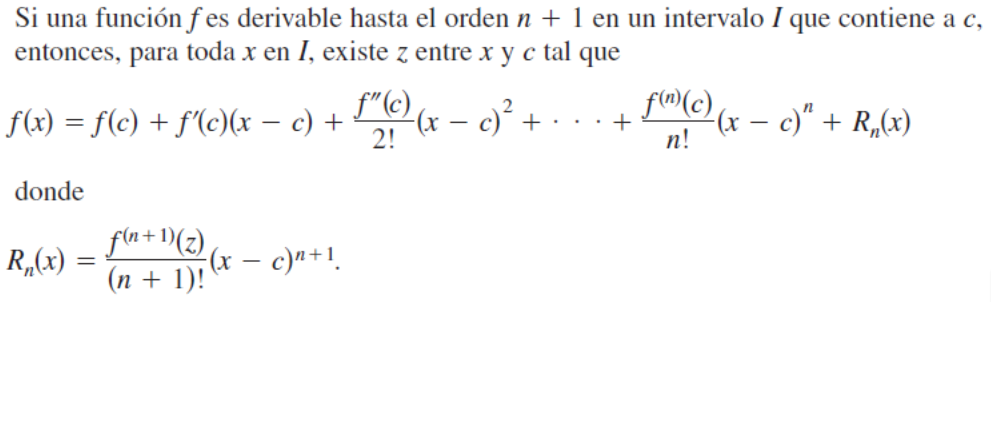
\includegraphics[width=\linewidth]{teorema_taylor.png}
      \caption {Teorema de Taylor}
      \label {fig:teorema_taylor}
    \end{figure}
    
    
    \section{Incidencia del centro en las aproximaciones}
        \subsection{procedimiento}
        Se tomo la funcion exponencial como funcion de prueba, para demostrar que entre mas 
        cerca se encuentren el centro y el resultado se necesitaran menos iteraciones para 
        hallar un valor mas preciso.
        Como se mostrara a continuacion se tomaron tres centros diferentes a para cada centro
        se encontro el polinomio de Taylor correspondiente luego de esto se evaluo el resultado
        con cinco iteraciones de tres valores diferentes cercanos a cada centro y al finalizar se
        analiza el numero de iteraciones requeridas para encontrar una aproximacion con cierta
        tolerancia.

        \subsubsection{polinomio de Taylor}
        La derivada


        \section {Ejemplos para aproximar valores de diferentes funciones}

        \section {Aproximaciones para combinaciones aritméticas de las funciones escogidas en el numeral 3}

        \section {Referencias}

        \begin{itemize}
        \item{Larson, R. and Edwards, B. (2010). Calculo 1 de una variable. 9th ed. Mexico. DF: McGraw Hill, pp.650-657.}
        \item{}
        \end{itemize}

\end{document}
